%!TEX root = ../main.tex

\chapter{Results}\label{cha:results}

\section{Interpretation of TFT}

\begin{figure}[hbtp!]
\centering
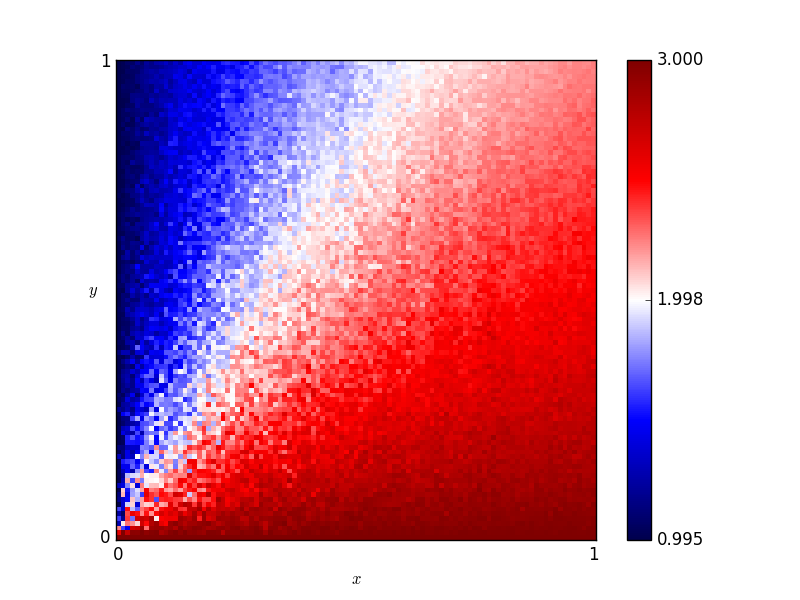
\includegraphics[width = 0.6\textwidth]{../img/Numerical/Tit_For_Tat.png}
\end{figure}


\section{Varying the parameter for Random}

\section{Alternator, Cycler(CD), Cooperator, Defector}

\section{GoByMajority for different parameters}

\begin{figure}[htbp!]
\subfloat[GoByMajority with memory depth 5]{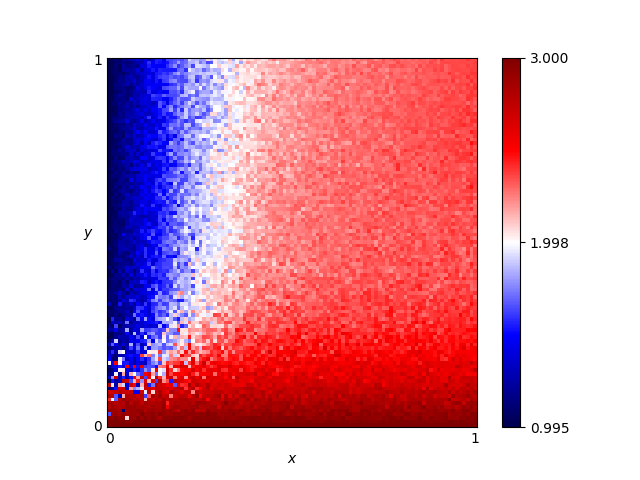
\includegraphics[width = 0.5\textwidth]{../img/Numerical/Go_By_Majority_5.png}}
\subfloat[GoByMajority with memory depth 10]{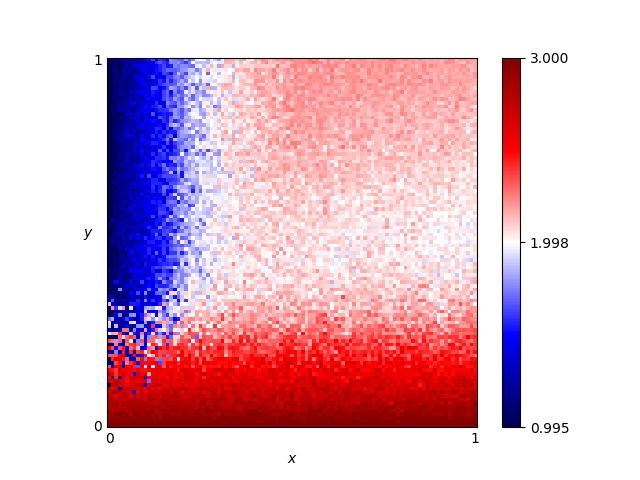
\includegraphics[width = 0.5\textwidth]{../img/Numerical/Go_By_Majority_10.png}}\\
\\
\subfloat[GoByMajority with memory depth 20]{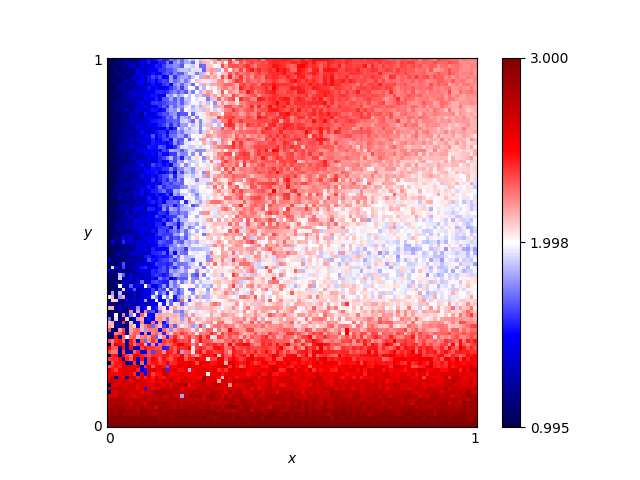
\includegraphics[width = 0.5\textwidth]{../img/Numerical/Go_By_Majority_20.png}}
\subfloat[GoByMajority with memory depth 40]{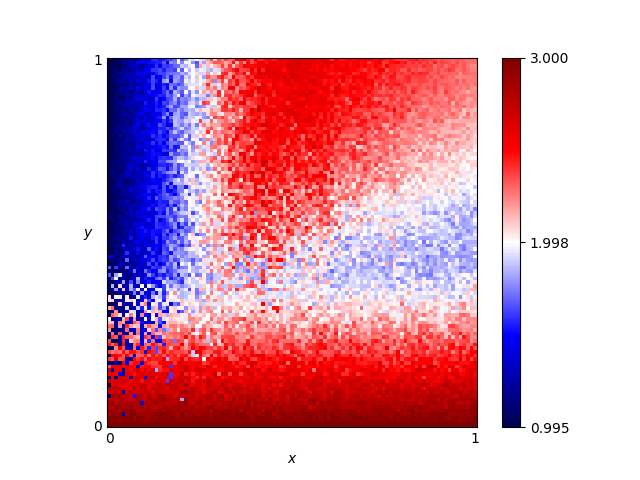
\includegraphics[width = 0.5\textwidth]{../img/Numerical/Go_By_Majority_40.png}}\\
\\
\subfloat[GoByMajority with memory depth infinite]{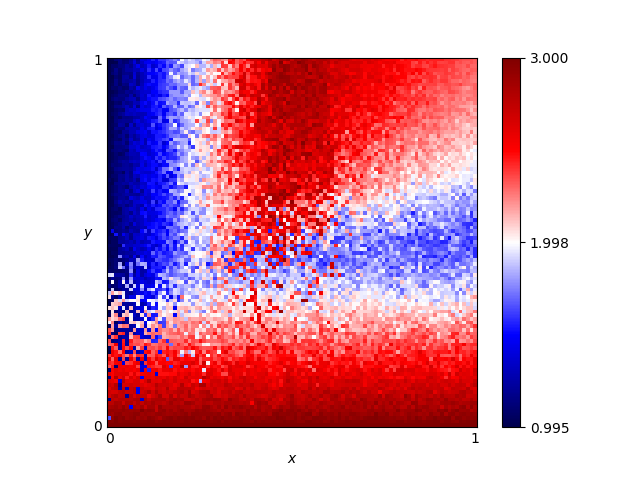
\includegraphics[width = 0.5\textwidth]{../img/Numerical/Go_By_Majority0.png}}

\end{figure}

\section{Random and Cycler(CDDC), TFT and T42T}

\section{LSE plot and table}
